\documentclass[conference]{IEEEtran}
\IEEEoverridecommandlockouts
% The preceding line is only needed to identify funding in the first footnote. If that is unneeded, please comment it out.
\usepackage{cite}
\usepackage{amsmath,amssymb,amsfonts}
\usepackage{algorithmic}
\usepackage{graphicx}
\usepackage{textcomp}
\usepackage{xcolor}
\def\BibTeX{{\rm B\kern-.05em{\sc i\kern-.025em b}\kern-.08em
    T\kern-.1667em\lower.7ex\hbox{E}\kern-.125emX}}
\begin{document}

\title{Performance Evaluation of Neural Networks for Intrusion Prevention Systems}

\author{\IEEEauthorblockN{Boris Stampf}
\IEEEauthorblockA{\textit{IT Security} \\
\textit{FH Technikum Wien}\\
Vienna, Austria\\
cs19m006@technikum-wien.at}
\and
\IEEEauthorblockN{Maximilian Wech}
\IEEEauthorblockA{\textit{IT Security} \\
\textit{FH Technikum Wien}\\
Vienna, Austria \\
cs19m020@technikum-wien.at}
}

\maketitle

\begin{abstract}
The detection of malicious behavior in network traffic through the use of machine learning algorithms in intrusion prevention systems is still a current topic of research. This paper focuses on neural networks and examines their performance across different datasets. Basically, the quality of the data with which machine learning algorithms are trained is a decisive factor for the classification performance. In addition to the publicly available CSE-CIC-IDS2018 dataset, this work also uses a dataset that was created with the help of feature extraction from automatically generated network traffic. Different scenarios are tested, but it turns out that the classification performance of neural networks in this context is only satisfactory if they are tested with data from the dataset with which they were trained. If another dataset is used for testing, the result of the classification is poor. This indicates that neural networks react sensitively to differences in the datasets and that the classification performance is influenced by this.
\end{abstract}

\begin{IEEEkeywords}
artificial intelligence, neural networks, computer networks, network security, feature extraction
\end{IEEEkeywords}

\section{Introduction}
The main goal of this paper is the comparison of a new dataset for intrusion prevention systems, which was created using automatically generated network traffic \cite{paper1}, with the CSE-CIC-IDS-2018 dataset \cite{max2}, using both a newly trained neural network and a neural network previously trained using the CSE-CIC-IDS-2018 dataset \cite{max1}. Because raw traffic network data cannot be used for training and classification using a neural network, meaningful features have to be extracted first. This process is described in Section \ref{extraction}. The extracted features can then be used for training and classification using multiple neural networks. This task is discussed and its results are shown in Section \ref{nn}. Finally, a conclusion based on these results is given in Section \ref{conclusion}.

\section{Feature Extraction}\label{extraction}
Before the neural network can be trained and used for classification, features have to be extracted from the raw network traffic data which was recorded in a previous step \cite{paper1}. For this task, the open-source Java software CICFlowMeter \cite{cicflowmeter} was chosen. The CICFlowMeter software was also used to create the CSE-CIC-IDS-2018 dataset \cite{max2}. This was a major reason for using it in this paper, as one of its goals is comparing the newly created dataset to the CSE-CIC-IDS2018 dataset. Some adaptations had to be made to the software, however, before it could be used to extract the desired features and also the labels from the recorded network traffic. Subsection \ref{extraction_using_cicflowmeter} describes how the CICFlowMeter in general extracts features from recorded network traffic. Subsection \ref{adaptation} then outlines the adaptations which had to be made.

\subsection{Extraction of flow-based features using CICFlowMeter}\label{extraction_using_cicflowmeter}
A common approach for extracting features from network traffic is to group packets into flows, and then calculate statistical features based on these flows. Because the CICFlowMeter software\cite{cicflowmeter} has been used used to fulfill that task for the creation of various datasets \cite{max2,sopuru,lashkari} and also during the creation of this paper, the following explanation is describing the functionality of that particular software. However, there is also a number of applications using various other software, also based on the idea of network-flow generation \cite{wang,moustafa,celik,waizumi}.

For each recorded packet read from a file in the \verb|pcap| format, the \verb|FlowGenerator| first checks if there is already a flow with that source IP address, destination IP address, source port, destination port and protocol (\verb|TCP| or \verb|UDP|). When this is the case, the packet information is added to that flow. Because CICFlowMeter is actually a bi-flow generator, the IP address and port of the source and destination may also be swapped, in which case the packet is regarded as a backwards packet. When no matching flow is found, a new flow is created (the first packet of each flow determines the forward and backward directions). A flow ends when a FIN packet is sent (TCP) or a configurable timeout occurs (UDP and TCP, 120 seconds by default), and the state of a flow changes from active to idle after a shorter timeout (default: five seconds). A flow is also divided into subflows whenever more than one second elapsed between two packets. The \verb|FlowGenerator| aggregates the information of each packet and calculates various statistical features. In addition to the features that define a flow (flow ID, IP address, port and protocol), CICFlowMeter supports a wide range of statistical features, including simple packet counts, totals, extrema (max, min), mean and standard deviation (Std). Some features, such as the inter-arrival-time (IAT, i.e. the time elapsed between two packets), are time-based, others depend on packet size, certain TCP flags and bulk (Blk) data flows. As the flows are bidirectional, the features can also distinguish between forward (Fwd) and backward (Bwd) directions. The full list of features supported by CICFlowMeter is given in Table \ref{table:cicflowmeter_features}, although the software is open-source and can therefore easily be extended to support currently disregarded features.

\begin{table}[htbp]
\caption{List of features supported by CICFlowMeter}
\begin{tabular}{| l l l |}
\hline
Flow ID & Src IP & Src Port \\
Dst IP & Dst Port & Protocol \\
Timestamp & Flow Duration & Tot Fwd Pkts \\
Tot Bwd Pkts & TotLen Fwd Pkts & TotLen Bwd Pkts \\
Fwd Pkt Len Max & Fwd Pkt Len Min & Fwd Pkt Len Mean \\
Fwd Pkt Len Std & Bwd Pkt Len Max & Bwd Pkt Len Mi \\
Bwd Pkt Len Mean & Bwd Pkt Len Std & Flow Bytes/s \\
Flow Pkts/s & Flow IAT Mean & Flow IAT Std \\
Flow IAT Max & Flow IAT Min & Fwd IAT Tot \\
Fwd IAT Mean & Fwd IAT Std & Fwd IAT Max \\
Fwd IAT Min & Bwd IAT Tot & Bwd IAT Mean \\
Bwd IAT Std & Bwd IAT Max & Bwd IAT Min \\
Fwd PSH Flags & Bwd PSH Flags & Fwd URG Flags \\
Bwd URG Flags & Fwd Header Len & Bwd Header Len \\
Fwd Pkts/s & Bwd Pkts/s & Pkt Len Min \\
Pkt Len Max & Pkt Len Mean & Pkt Len Std \\
Pkt Len Var & FIN Flag Cnt & SYN Flag Cnt \\
RST Flag Cnt & PSH Flag Cnt & ACK Flag Cnt \\
URG Flag Cnt & CWE Flag Count & ECE Flag Cnt \\
Down/Up Ratio & Pkt Size Avg & Fwd Seg Size Avg \\
Bwd Seg Size Avg & Fwd Byts/b Avg & Fwd Pkts/b Avg \\
Fwd Blk Rate Avg & Bwd Byts/b Avg & Bwd Pkts/b Avg \\
Bwd Blk Rate Avg & Subflow Fwd Pkts & Subflow Fwd Byts \\
Subflow Bwd Pkts & Subflow Bwd Byts & Init Fwd Win Byts \\
Init Bwd Win Byts & Fwd Act Data Pkts & Fwd Seg Size Min \\
Active Mean & Active Std & Active Max \\
Active Min & Idle Mean & Idle Std \\
Idle Max & Idle Min & \\
\hline
\end{tabular}
\label{table:cicflowmeter_features}
\end{table}

The CICFlowMeter has a command-line interface (which can be accessed by executing the Java main class \verb|cic.cs.unb.ca.ifm.Cmd|) and a graphical user interface (GUI, \verb|cic.cs.unb.ca.ifm.CICFlowMeter|). The command-line interface takes two parameters: the name of the input file (in \verb|pcap| format) or directory (in that case, all pcap files in that directory are read) and the name of the output directory. For each pcap file which was read, a separate comma-separated values (csv) file containing the extracted features is written to the output directory. The GUI allows to adjust additional parameters, such as the flow timeouts (see Figure \ref{fig:cicflowmeter_offline}), and is able to extract features in realtime by directly listening to a network interface (see Figure \ref{fig:cicflowmeter_realtime}).

\begin{figure}[htbp]  
\centerline{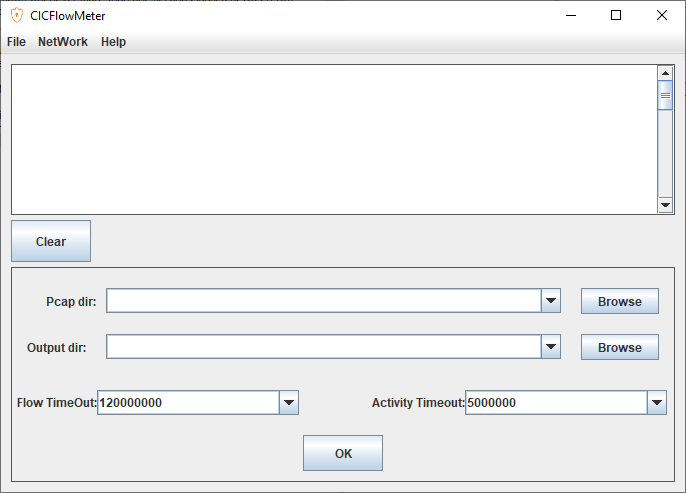
\includegraphics[scale=0.45]{CICFlowMeterOffline.png}}
\caption{CICFlowMeter GUI (offline mode)}
\label{fig:cicflowmeter_offline}
\end{figure}

\begin{figure}[htbp]  
\centerline{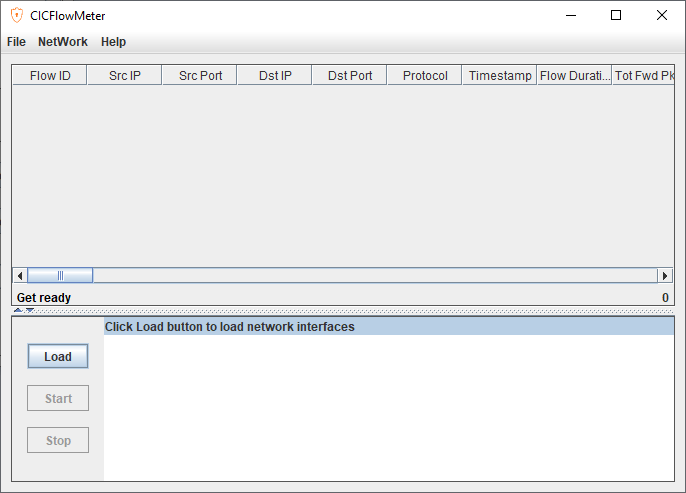
\includegraphics[scale=0.45]{CICFlowMeterRealtime.png}}
\caption{CICFlowMeter GUI (realtime mode)}
\label{fig:cicflowmeter_realtime}
\end{figure}

\subsection{Adaptation of the CICFlowMeter software}\label{adaptation}
Because the CICFlowMeter is open-source software available at GitHub \cite{cicflowmeter_github} and written in Java, it could easily be extended for the requirements of this paper.

The biggest change was necessary because of the way how the labelling was achieved. To ensure both accuracy and flexibility, the network traffic resulting from each host was recorded separately, resulting in multiple files in the pcap format \cite{paper1}. The label is defined by the file name: if the file name starts with an attack type label, that label is assigned to it - otherwise, its contents are labelled as benign network traffic. For this reason, the command-line interface of the CICFlowMeter was extended. It now retrieves a list of attack type labels, separated by a colon (e.g. \verb|ssh-bruteforce:bot:dos-goldeneye|) as an additional command-line parameter. It then reads the contents of the input directory specified in another command-line parameter and opens every file in it which name ends with \verb|.pcap|. So, instead of reading one file at a time as in the original implementation, multiple instances of the class \verb|cic.cs.unb.ca.jnetpcap.PacketReader| are created (one for each pcap file in the input directory), and assigned a label depending on the file name. Then, the information of the first valid packet is read from each \verb|PacketReader|. In the next step, the timestamps of these packets are compared, and the packet with the lowest timestamp (i.e. the earliest) is sent to a single \verb|FlowGenerator| instance. The only change made to the \verb|FlowGenerator| implementation is that it now takes the label as a parameter and forwards it to the \verb|BasicFlow| instance. The \verb|BasicFlow| keeps track of how many packets per label were found, and then sets the label of the flow accordingly: if all packets of that flow are benign, the label is set to \verb|BENIGN|, otherwise it is set to the attack type label with the highest packet count. After processing the packet data, the next packet from the same \verb|PacketReader| is read. Afterwards, the determination of the packet with the lowest timestamp is repeated, and its contents are also sent to the \verb|FlowGenerator|. When the end of file (EOF) has been reached for any pcap file, the corresponding \verb|PacketReader| is no longer considered, and the process continues with the remaining \verb|PacketReader| instances. This is repeated until all packets from all opened pcap files have been read.

Another change was made in order to efficiently use the newly created dataset with the neural network from \cite{max1}. For that reason, and to achieve as much flexibility as possible, another command-line parameter was added to the CICFlowMeter. This parameter lists all features which should be extracted (as with the attack labels, separated by a colon). The function which writes the flow features to the resulting \verb|csv| file was extended and now retrieves the list of flow features, which is passed from the newly added command-line parameter. Instead of writing all features supported by the CICFlowMeter, it now writes only the desired features, in the exact order they were specified. Of course, this also has to be considered when writing the headers to the first line of the \verb|csv| file (these list the names of the features). The new parameter allows the data to be extracted in a way that does not unnecessarily complicate the preprocessing of the neural network. If the parameter is ommitted, all features are written to the \verb|csv| file, exactly as in the original version of the CICFlowMeter.

For optimal integration into the infrastructure created in \cite{paper1}, a Docker image for feature extraction was created. For reasons of efficiency, the \verb|Dockerfile| used to create that image was written so that it employs a multi-stage build \cite{docker-multistage}. The first stage uses the image \verb|gradle:6.3.0-jdk11| (the Gradle and Java versions are set explicitly to ensure compatibility with the CICFlowMeter source code) from Docker Hub \cite{dockerhub}, copies the modified CICFlowMeter source code from the build context (in this case this is the directory that the \verb|Dockerfile| is contained in) into a temporary image and runs \verb|gradle| to build the CICFlowMeter distribution. The second stage is based on the image \verb|azul/zulu-openjdk:11| (again, the Java version is set explicitly). It runs \verb|jlink| \cite{jlink} to create a minimal Java 11 Runtime Environment containing only the modules required by the CICFlowMeter, which is written to another temporary image. Finally, the last stage builds the actual feature extraction Docker image. It is based on \verb|ubuntu:latest|, installs the \verb|libpcap| library required by the CICFlowMeter and copies the Java Runtime Environment and the CICFlowMeter distribution from the temporary images created in the previous stages. The \verb|ENTRYPOINT| of the docker image is set to the Java Virtual Machine binary, and all command-line parameters which are required to run the command-line interface of the CICFlowMeter are set as well. The data directory is set to \verb|/mnt/packet-data|, which means that the external directory containing all the pcap files has to be mounted to that directory of the Docker container. The \verb|csv| file with the extracted features is also written to that directory. Another dependency required by the Docker container is the environment variable \verb|ATTACKS|, which has to contain the attack labels separated by a colon. The list of features is read from the environment variable \verb|FEATURES|. When this environment variable is missing, all supported features are extracted.

\section{Neural Network}\label{nn}
The created dataset will be used in the further course of this paper to build a neural network. With this it should be possible to detect anomalies in network traffic (e. g. DoS attacks) but also harmless data packets. This is a continuation of  \cite{max1}, in which an attempt was made to create a neural network for intrusion detection on the basis of the publicly available CSE-CIC-IDS2018 dataset  \cite{max2}. The knowledge gained at that time is used, the source codes are reused accordingly and slightly adapted to the new dataset. In principle, the performance of neural networks over different datasets is to be checked. The following scenarios will be considered:
\smallskip

Scenario 1) What performance can be achieved with a neural network when it is trained and tested with the dataset created in this work? 
\smallskip

Scenario 2) How well does the neural network created in Scenario 1 work when tested with the CSE-CIC-IDS2018 dataset  \cite{max2}? 
\smallskip

Scenario 3) How well does the neural network trained in \cite{max1} work when tested with the dataset created in this work?
\smallskip

It is expectable that there are differences in intrusion detection or -prevention datasets because, for example, cyber attacks are not always executed or recorded in the same way or the network infrastructure is structured differently. The aim is to determine how sensitive neural networks react to this and are thus dependent on the data with which they have been trained. This chapter is designed in such a way that the various steps for building up the neural network are first described and then the results obtained are examined in detail.

\subsection{Setup}
For the practical implementation, a notebook with 16GB RAM and a 2.7 GHz dual-core processor was used. This hardware was sufficient for the fulfillment of the task. The training of the neural network took about 4 hours. PyCharm Community Edition 2020.1 was used as a Python development environment on Windows 10. Packages were basically the same as in \cite{max1}. The Seaborn package 0.10.1 was also used to create heatmaps.

\subsection{Preprocessing}
This process is based on the one from\cite{max1}. This involves preparing the created dataset for training the neural network accordingly. A difference compared to \cite{max1} is that this time no headers were in the middle of the created CSV file. For this reason, the "skip\_rows" parameter did not have to be used in the "read\_csv" pandas function. In addition, identical entries in the dataset (duplicates) are also removed and a corresponding data type is specified for each feature. The conversion of the labels into a numeric format also takes place. At this point it should be noted that due to time constraints, not all types of attack from \cite{max2} could be reproduced in this work. This can be seen from the fact that some (numerical) labels are not represented in the created dataset. In the context of future work, the missing types of attack can be added. It is important that the labels in the created dataset must have the exact same numerical representation as in \cite{max1}. This means, for example, that benign network traffic must be labeled with "0" again. Furthermore, no types of attack were implemented in the context of this work that are not available in the CSE-CIC-IDS2018 dataset \cite{max2}. This is because the neural network from \cite{max1} could not recognize them and thus no performance comparison would be possible. For this reason, attacks from the CSE-CIC-IDS2018 dataset \cite{max2} were selectively reproduced. It should also be noted that in \cite{max1} some attacks of the publicly available dataset were not included.

\smallskip
The following Table \ref{table:overviewdatasets} provides an overview of both datasets:
\begin{table}[htbp]
\caption{Overview of the two datasets } 
\centering
\begin{tabular}{ | c | c | c | }
\hline
Label & \multicolumn{1}{|p{2cm}|}{\centering Number of data \\ points in the dataset  \\ created in this work}  & \multicolumn{1}{|p{2cm}|}{\centering Number of data \\ points in the \\  CSE-CIC-IDS2018 dataset \cite{max2}}\\
\hline
benign (0) & 63.264 & 10.180.908 \\
\hline
ddos attacks-loic-http (1) & Not available & 575.364 \\
\hline
ddos attack-hoic (2) & 193.729	& 198.861 \\
\hline
dos attacks-hulk (3) & Not available & 145.199 \\
\hline
bot (4) & Not available & 144.535 \\
\hline
ssh-bruteforce (5) & 29.182 & 94.048 \\
\hline
dos-goldeneye (6) & 7.368.370	 & 41.406 \\
\hline
dos attacks-slowloris (7) & Not available & 9.908 \\
\hline
ddos attack-loic-udp (8) & Not available & 1.730 \\
\hline
\end{tabular}
\label{table:overviewdatasets}
\end{table}

While the CSE-CIC-IDS2018 dataset \cite{max2} has a total of 10,182,638 data points (6.41GB distributed over multiple CSV files), the dataset created in this work consists of 7,654,545 data points (4.1GB, only one CSV file). When looking at Table 1, it is noticeable that both datasets are unbalanced and there is one label for which comparatively many data points exist (dataset created in this work: "dos-goldeneye", CSE-CIC-IDS2018 dataset: "benign").
The preprocessing process of the final dataset takes about 10 minutes. This is comparatively faster than in \cite{max1}, which could be due to the smaller file size and the fact that the current dataset consists of only one CSV file (there is no need to merge several files). Finally, the dataset was divided into a training and a test set at a ratio of 80:20. While the former is used to train the neural network, the latter is used to determine the performance of the neural network (with data not used for training).

\subsection{Training the neural network}
After the preprocessing of the data has been completed, the next task is to train and test the neural network. The architecture recommended in \cite{max1} (three hidden layers with 69 neurons each) and the hyperparameters (Learn rate: 0. 0001, Optimizer: adam, Weight initialization: normal, Activation function: relu, Number of neurons per layer: 69, Epochs: 850, Batch size: 256) are reused. In addition, "MinMaxScale" was used to normalize the data and a weight value of 500 was set for benign traffic. At this point it is worth mentioning that attempts have been made to adjust individual parameters such as the learn rate or the weight value of benign traffic in order to achieve a better result. However, this has not had any positive effects. Future work could deal with this in more detail and try to find optimal hyperparameters by an extensive gridsearch. Of course, this would require appropriate hardware resources.

\smallskip
Training of the neural network with the training set took 4 hours and was stopped after 129 epochs. As in \cite{max1}, "EarlyStopping" with a value of 50 epochs was used. This means that after 50 epochs without improvement, the learning process is terminated to avoid overfitting.

\subsection{Results}
In the further course of this chapter, the aim is to present and evaluate the results achieved. To determine how good the classifications of machine learning algorithms are, an appropriate measure is required. The following metrics are relevant \cite{max3}:
\smallskip 

Accuracy: How likely is the model to make a correct prediction?
\smallskip

Precision for class A: How likely is the classification to be correct if the model predicts class A?
\smallskip

Recall for class A: How much data of a class A can the model correctly predict?
\smallskip

Both the dataset created in this work and the CSE-CIC-IDS2018 dataset \cite{max2} are unbalanced (different amounts of data per class). For this reason, the use of Accuracy does not seem to be appropriate. If a very large amount of data were available for a class A and not for classes B and C, then the accuracy would be very dependent on class A. Instead, it is advisable to graphically display the classification results of the neural network in a confusion matrix and to calculate precision and recall respectively. The following text analyses the results of the three scenarios in the introduction:
Figure  \ref{fig:cm1} shows the result of the first scenario in which a neural network was trained and tested with the dataset created in this work. The classification results are largely good. However, it is noticeable, that only 62.5\% of all data of the "ssh-bruteforce" attack type can be correctly classified (comparatively low recall). The precision value for "benign" traffic is also comparatively lower, which means that it is only 86\% correct if the neural network predicts this class. All other precision and recall values are well over 95\%.

\begin{figure}[htbp]  
\centerline{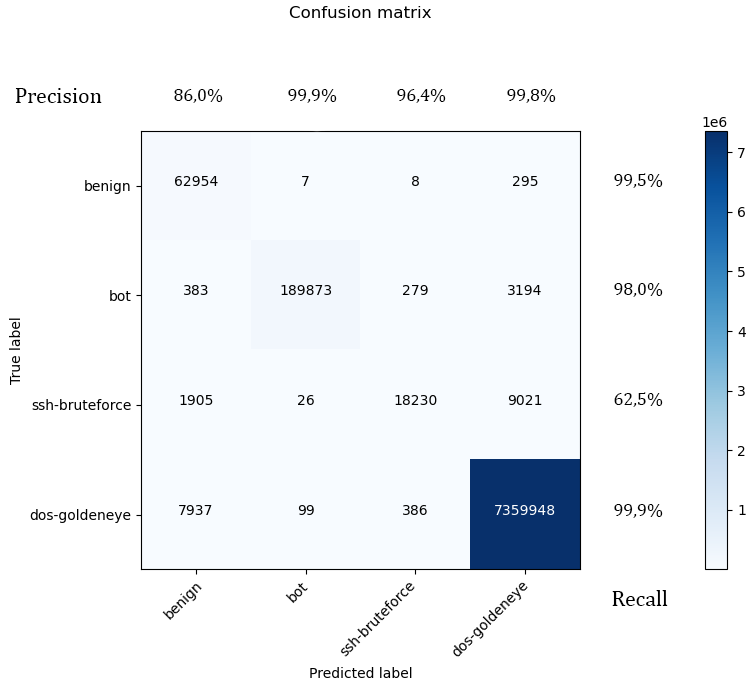
\includegraphics[scale=0.65]{NeuesModellNeueDaten.png}}
\caption{Confusion Matrix for Scenario 1}
\label{fig:cm1}
\end{figure}

Next, the neural network trained in Scenario 1 was reused and tested with the CSE-CIC-IDS2018 dataset \cite{max2}. There are many more classes (attack types) in this dataset than in the one used to train the neural network. Thus, the model would not be able to recognize these classes. For this reason, it is necessary to reduce the CSE-CIC-IDS2018 dataset \cite{max2} to the known four classes ("benign", "bot", "ssh-bruteforce" and "dos-goldeneye"). The reduced dataset is then used to test the neural network. The Confusion Matrix in Figure  \ref{fig:cm2} shows that the classification result is anything but good. On the positive side, the precision for benign traffic is very high, so if the model predicts this class, the prediction is 99.4\% correct. However, only 24.2\% of all data in this class can be correctly predicted. All other precision and recall values are or move around 0\%. It is worth mentioning that the "ssh-bruteforce" attack cannot be recognized correctly once. Scenario 1 already indicated a worse classification result for this class. Both "bot"- and "dos-goldeneye" attacks could be detected at least a few times, but to a very small extent. Overall, this suggests that there may be differences in the two datasets that significantly affect the classification outcome of the neural network. Thus, there is a suspicion that the machine learning model is overfitting.

\begin{figure}[htbp]  
\centerline{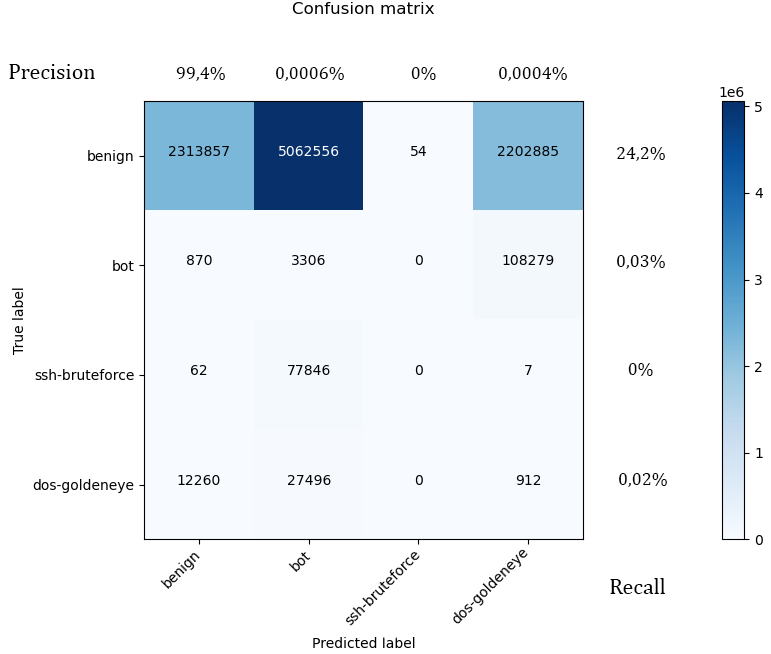
\includegraphics[scale=0.65]{NeuesModellAlteDaten.png}}
\caption{Confusion Matrix for Scenario 2}
\label{fig:cm2}
\end{figure}

In the third scenario, the neural network from \cite{max1}, which was trained with CSE-CIC-IDS2018 Dataset \cite{max2}, is now tested with the dataset of this work. This continues the low classification success (see Figure \ref{fig:cm3}). In the class "benign", 99.8\% of all data are correctly predicted (recall), but the precision is noticeably low (0. 008\%). This means that the neural network recognizes many data points as "benign", but these are mostly other classes. Conversely, this is the case with "bot", where only few data of this class are correctly recognized, but whenever the neural network recognizes this class, it is a correct prediction. All other precision and recall values are or move around 0\%. It is particularly noticeable that "bot"-, "ssh-bruteforce"- and "dos-goldeneye" attacks are mostly classified as benign traffic. Furthermore, it can be seen that "ssh-bruteforce"- and "dos-goldeneye" attacks cannot be correctly detected once; bot attacks can be correctly predicted nine times in total. This makes it clear how weak the classifications of the neural network trained in \cite{max1} are with the dataset created in this work. Also worth mentioning is that for some data points the classes "ddos attacks-loic-http", "dos attacks-hulk" and "dos attacks-slowloris" are predicted. These are not available in the dataset created in this work, but in the CSE-CIC-IDS2018 dataset \cite{max2}, with which the neural network was trained. For this reason, this is not surprising.

\begin{figure}[htbp]  
\centerline{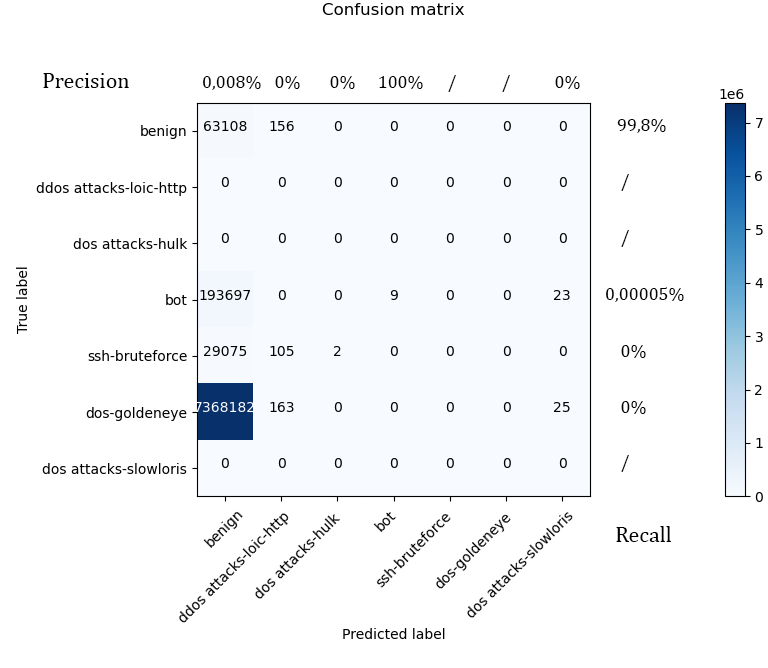
\includegraphics[scale=0.65]{AltesModellNeueDaten.png}}
\caption{Confusion Matrix for Scenario 3}
\label{fig:cm3}
\end{figure}

Scenarios 2 and 3 show that if in this context a neural network is tested with a different dataset than the one it was trained with, then the classification performance is poor. There can be many reasons for this. The suspicion, however, is that there are differences in the datasets and that this affects the predictions of the neural networks. One approach is to perform a correlation analysis. This makes it possible to determine the statistical relationship between two features (variables) of a dataset. The correlation coefficient is to be calculated, which indicates the strength of the correlation in the interval [-1.1]. A positive correlation means the larger the variable A, the larger the variable B. The opposite is the negative correlation, in which the larger the variable A is, the smaller the variable B. If the correlation coefficient is 0, this is called a neutral correlation and there is no relationship between the variables \cite{max4}. The idea is to determine the correlation between the features (variables) for each dataset individually. From this, graphical representations (heatmaps \cite{max5}) can be created in order to be able to compare whether correlation differences can be detected in the datasets. Since the number of features is high in both datasets, it makes sense to use only a subset of the features for the analysis. Thus, the correlation between the first 36 features is determined for both datasets. Figure \ref{fig:hm1} and Figure \ref{fig:hm2} each show the results for the two datasets. Clear differences are recognizable. It is worth mentioning that Figure \ref{fig:hm1} shows numerous negative correlations, which are not at all or hardly recognizable in Figure \ref{fig:hm2}. It is also noticeable that in Figure \ref{fig:hm2}, white lines occur, meaning that a feature in the dataset created in this work always has a value of zero. This shows that there are differences in the datasets. 

\begin{figure}[htbp]  
\centerline{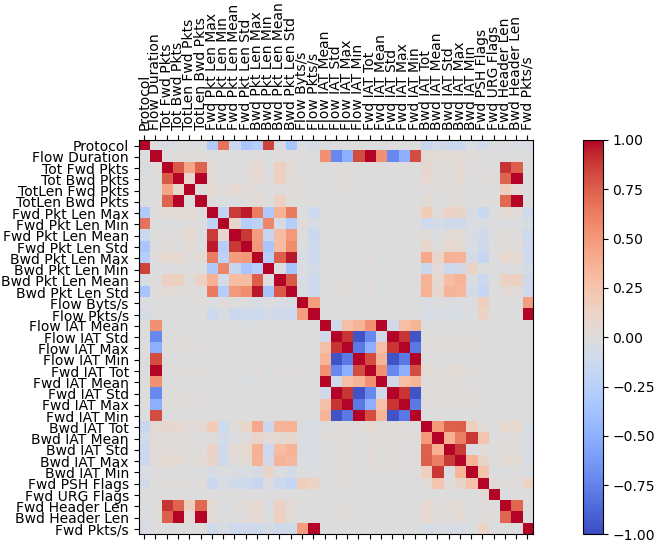
\includegraphics[scale=0.8]{Heatmap-AlteDaten-Filtered-0-35.png}}
\caption{Heatmap of the first 36 features of the CSE-CIC-IDS2018 Dataset}
\label{fig:hm1}
\end{figure}

\begin{figure}[htbp]  
\centerline{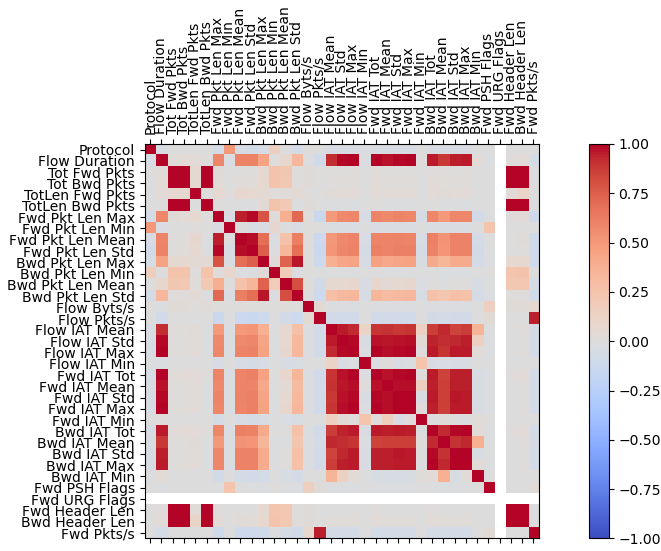
\includegraphics[scale=0.8]{Heatmap-NeueDaten-0-35.png}}
\caption{Heatmap of the first 36 features of the dataset created in this work}
\label{fig:hm2}
\end{figure}

\newpage

\section{Conclusion}\label{conclusion}
In summary, the performance of neural networks in terms of intrusion prevention over different datasets is rather mixed. If these machine learning algorithms are tested with the same dataset with which they were trained, the result is promising. Using another dataset for testing results in a poor classification performance. However, there is lots of potential for future research with neural networks in this context. It seems useful to analyse in detail why the mentioned difficulties occur in the classification and which factors are relevant for the neural network. An intensive examination of the finding of optimal hyperparameters would also be desirable in the course of future work. Furthermore, it would also make sense to simplify the way classification is done. Instead, a simple classification like network traffic is “benign” or “not benign” would be conceivable. Moreover, it should be checked whether a better performance can be achieved with other machine learning algorithms.

\begin{thebibliography}{00}
\bibitem{paper1} B. Gally, S. Lipp and D. Marijanovic, "Automated Network Packet Generation for Evaluation of Neural Networks in Intrusion Prevention Systems", FH Technikum, Vienna, 30 June 2020.
\bibitem{max2} I. Sharafaldin, A. H. Lashkari and A. A. Ghorbani, "Toward Generating a New Intrusion Detection Dataset and Intrusion Traffic Characterization", in 4th International Conference on Information Systems Security and Privacy (ICISSP), Portugal, 2018.
\bibitem{max1} F. Ahrens, C. Cat and R. Freingruber, "A Neural-Network Approach for an Intrusion Detection System", FH Technikum, Vienna, 2019.
\bibitem{cicflowmeter} Canadian Institute for Cybersecurity (CIC), "Applications | Research | Canadian Institute for Cybersecurity | UNB", 2016. [Online]. Available: https://www.unb.ca/cic/research/applications.html\#CICFlowMeter. [Accessed 29 June 2020].
\bibitem{sopuru} J. Sopuru, A. Sari and M. Akkaya, "Modeling a malware detection and categorization system based on seven network flow-based features", in International Journal of Innovative Technology and Exploring Engineering (IJITEE), vol. 8(7), pp. 2982-2989, 05 2019
\bibitem{lashkari} A. H. Lashkari, G. D. Gil, M. S. I. Mamun and A. A. Ghorbani, "Characterization of tor traffic using time based features", in Proceedings of the 3rd International Conference on Information Systems Security and Privacy (ICISSP 2017), pp. 253-262, 2017.
\bibitem{wang} W. Wang, Y. Sheng, J. Wang, X. Zeng, X. Ye, Y. Huang and M. Zhu, HAST-IDS: Learning hierarchical spatial-temporal features Using deep neural networks to improve intrusion detection. IEEE Access, vol. 6, pp. 1792-1806, 2018.
\bibitem{moustafa} N. Moustafa and J. Slay, "UNSW-NB15: a comprehensive data set for network intrusion detection systems (UNSW-NB15 network data set)", in 2015 Military Communications and Information Systems Conference (MilCIS), Canberra, ACT, 2015, pp. 1-6.
\bibitem{celik} Z. Celik, Berkay, R. J. Walls, P. McDaniel and A. Swami, "Malware traffic detection using tamper resistant features", in MILCOM 2015 - 2015 IEEE Military Communications Conference, pp. 330–335, Oct 2015.
\bibitem{waizumi} Y. Waizumi, Y. Sato and Y. Nemoto, "A network-based anomaly detection system using multiple network features", in Proceedings of the Third International Conference on Web Information Systems and Technologies - Internet Technology, pp. 410-413, 2007.
\bibitem{cicflowmeter_github} GitHub - ahlashkari/CICFlowMeter: CICFlowmeter-V4.0 (formerly known as ISCXFlowMeter) is an Ethernet traffic Bi-flow generator and analyzer for anomaly detection that has been used in many Cybersecurity datsets such as Android Adware-General Malware dataset (CICAAGM2017), IPS/IDS dataset (CICIDS2017), Android Malware dataset (CICAndMal2017) and Distributed Denial of Service (CICDDoS2019). [Online]. Available: https://github.com/ahlashkari/CICFlowMeter. [Accessed 29 June 2020].
\bibitem{docker-multistage} Use multi-stage builds | Docker Documentation. [Online]. Available: https://docs.docker.com/develop/develop-images/multistage-build/. [Accessed 29 June 2020].
\bibitem{dockerhub} Docker Hub. [Online]. Available: https://hub.docker.com/. [Accessed 29 June 2020].
\bibitem{jlink} The Incredible Shrinking Java Platform - Azul Systems, Inc.. [Online]. Available: https://www.azul.com/blog/the-incredible-shrinking-java-platform/. [Accessed 29 June 2020].
\bibitem{max3} D. Meyer, "Performance Assessment \& Tuning - Presentation slides", FH Technikum, Vienna, 2018.
\bibitem{max4} J. Brownlee, "How to Calculate Correlation Between Variables in Python", 3 June 2020. [Online]. Available: https://machinelearningmastery.com/how-to-use-correlation-to-understand-the-relationship-between-variables/. [Accessed 27 June 2020].
\bibitem{max5} S. Norena, "Finding Correlation Between Many Variables (Multidimensional Dataset) with Python", 26 April 2018. [Online]. Available: https://medium.com/@sebastiannorena/finding-correlation-between-many-variables-multidimensional-dataset-with-python-5deb3f39ffb3. [Accessed 27 June 2020].
\end{thebibliography}

\end{document}